\documentclass[ignorenonframetext,]{beamer}
\setbeamertemplate{caption}[numbered]
\setbeamertemplate{caption label separator}{: }
\setbeamercolor{caption name}{fg=normal text.fg}
\beamertemplatenavigationsymbolsempty
\usepackage{lmodern}
\usepackage{amssymb,amsmath}
\usepackage{ifxetex,ifluatex}
\usepackage{fixltx2e} % provides \textsubscript
\ifnum 0\ifxetex 1\fi\ifluatex 1\fi=0 % if pdftex
\usepackage[T1]{fontenc}
\usepackage[utf8]{inputenc}
\else % if luatex or xelatex
\ifxetex
\usepackage{mathspec}
\else
\usepackage{fontspec}
\fi
\defaultfontfeatures{Ligatures=TeX,Scale=MatchLowercase}
\fi
\usetheme{Madrid}
\usecolortheme{udesc}
% use upquote if available, for straight quotes in verbatim environments
\IfFileExists{upquote.sty}{\usepackage{upquote}}{}
% use microtype if available
\IfFileExists{microtype.sty}{%
\usepackage{microtype}
\UseMicrotypeSet[protrusion]{basicmath} % disable protrusion for tt fonts
}{}
\newif\ifbibliography
\usepackage{graphicx,grffile}
\makeatletter
\def\maxwidth{\ifdim\Gin@nat@width>\linewidth\linewidth\else\Gin@nat@width\fi}
\def\maxheight{\ifdim\Gin@nat@height>\textheight0.8\textheight\else\Gin@nat@height\fi}
\makeatother
% Scale images if necessary, so that they will not overflow the page
% margins by default, and it is still possible to overwrite the defaults
% using explicit options in \includegraphics[width, height, ...]{}
\setkeys{Gin}{width=\maxwidth,height=\maxheight,keepaspectratio}

% Prevent slide breaks in the middle of a paragraph:
\widowpenalties 1 10000
\raggedbottom

\AtBeginPart{
\let\insertpartnumber\relax
\let\partname\relax
\frame{\partpage}
}
\AtBeginSection{
\ifbibliography
\else
\let\insertsectionnumber\relax
\let\sectionname\relax
\frame{\sectionpage}
\fi
}
\AtBeginSubsection{
\let\insertsubsectionnumber\relax
\let\subsectionname\relax
\frame{\subsectionpage}
}

\setlength{\parindent}{0pt}
\setlength{\parskip}{6pt plus 2pt minus 1pt}
\setlength{\emergencystretch}{3em}  % prevent overfull lines
\providecommand{\tightlist}{%
\setlength{\itemsep}{0pt}\setlength{\parskip}{0pt}}
\setcounter{secnumdepth}{0}
%%%%%%%%%%%%%%%%%%%%%%%%%%%%%%%%%%%%%%%%%%%%%%%%%%%%%%%%%%%%%%%%%%%%%%%%%%%%%%%%%%%%%%%%%%%%%%
% Template Beamer 
% Based on MIT Beamer Template e Senac
% Cores verde e vermelho tentam seguir o padrão visual da Udesc
%%%%%%%%%%%%%%%%%%%%%%%%%%%%%%%%%%%%%%%%%%%%%%%%%%%%%%%%%%%%%%%%%%%%%%%%%%%%%%%%%%%%%%%%%%%%%% 

\usepackage{graphicx,url}
\usepackage{tikz}
\usepackage[brazil]{babel}   
\usepackage{textpos}
\usepackage{transparent}

\batchmode
% \usepackage{pgfpages}
% \pgfpagesuselayout{4 on 1}[letterpaper,landscape,border shrink=5mm]
\usepackage{amsmath,amssymb,enumerate,epsfig,bbm,calc,color,ifthen,capt-of}

%-------------------------Declara figura do Logo-----------------------------------------------------
\pgfdeclareimage[height=0.8cm]{Marca_Udesc}{Marca_Udesc.pdf}
%\logo{\pgfuseimage{Marca_Udesc}\vspace*{7.0cm}}


%% ------------------ Figura de fundo do slide de titulo
%\setbeamercolor{titlelike}{parent=structure}
%\makeatletter
%\setbeamertemplate{title page}
%{
%	\begin{tikzpicture}[remember picture, overlay]
%	\node[at=(current page.center)]{
%		
\includegraphics[width=\paperwidth, height=\paperheight]{risk1.jpg}	
%	};
%	\end{tikzpicture}
%	%	\vbox{}
%	%	\vfill
%	%	\begingroup
%	%	\centering
%	%	\pgfsetfillopacity{0.1}
%	%	\setbeamercolor{title}{bg=black}
%	%	\begin{beamercolorbox}[sep=8pt,center]{title}	
%	%		\usebeamerfont{title}\inserttitle\par%
%	%		\ifx\insertsubtitle\@empty%
%	%		\else%
%	%		\vskip0.25em%
%	%		{\usebeamerfont{subtitle}\usebeamercolor[fg]{subtitle}\insertsubtitle\par}%
%	%		\fi%
%	%	\end{beamercolorbox}%
%	\begin{textblock*}{0.8\textwidth}(2.5em, -2.5em)
%		\centering
%		\setbeamerfont{title}{size=\Huge}
%		{\usebeamerfont{title}\usebeamercolor[bg]{title}\inserttitle\par}%
%	\end{textblock*}
%	%	\vskip3em\par
%	%	\begin{beamercolorbox}[sep=8pt,center]{author}
%	%		\usebeamerfont{author}\insertauthor
%	%	\end{beamercolorbox}
%	%	\begin{beamercolorbox}[sep=8pt,center]{institute}
%	%		\usebeamerfont{institute}\insertinstitute
%	%	\end{beamercolorbox}
%	%	\begin{beamercolorbox}[sep=8pt,center]{date}
%	%		\usebeamerfont{date}\insertdate
%	%	\end{beamercolorbox}\vskip0.5em
%	%	\endgroup
%	\vfill
%}
%\makeatother

%Global Background must be put in preamble
%\usebackgroundtemplate%
%{%
%	\transparent{0.2}
\includegraphics[width=\paperwidth,height=\paperheight]{risk-management.jpg}%
%}


%-------------------------Este código faz o menuzinho bacana na parte superior do slide------------
\AtBeginSection[]
{
%  \begin{frame}<beamer>
%    \frametitle{Sumário}
%    \tableofcontents[currentsection]
%  \end{frame}
}

\AtBeginSubsection{}

% Para ativar os tópicos de forma incremental
%\beamerdefaultoverlayspecification{<+->}
% -----------------------------------------------------------------------------
% -----Página de título sem o logo -----------------------------------
%\renewcommand{\titlepage}{\setbeamertemplate{logo}{}\titlepage}
%\setbeamertemplate{logo}{}\titlepage

% ------------ Logo na parte superior direita --------------------------------
\addtobeamertemplate{frametitle}{}{%
\begin{textblock*}{100mm}(.85\textwidth,-0.9cm)
\pgfuseimage{Marca_Udesc}
\end{textblock*}}
%
% - Para criar duas colunas em algum slide da apresentacao 
% - a partir do Rmarkdown
\def\begincols{\begin{columns}}
\def\begincol{\begin{column}}
\def\endcol{\end{column}}
\def\endcols{\end{columns}}

%%---Gerador de Sumário---------------------------------------------------------
%\section[]{}
%\begin{frame}{Sumário}
%  \tableofcontents
%\end{frame}
%---Fim do Sumário------------------------------------------------------------

\title[Mercado de Capitais]{Medidas condicionais de risco com teoria do valor extremo}
\author{Rafael Felipe Bressan}
\date{22-11-2017}

\begin{document}
\frame{\titlepage}

%%------------------------------------------------------------------------------
%% Before Body
%%------------------------------------------------------------------------------
%%---Gerador de Sumário---------------------------------------------------------
\section[]{}
\begin{frame}{Sumário}
  \tableofcontents
\end{frame}
%---Fim do Sumário------------------------------------------------------------

\section{Introdução}\label{introducao}

\begin{frame}{Motivação}

\begin{itemize}
\tightlist
\item
  De acordo com os princípios do acordo de Basileia III, as instituições
  financeiras supervisionadas pelos Bancos Centrais devem manter
  \emph{buffers} de capital contra riscos de mercado, crédito, liquidez,
  entre outros.
\item
  Para riscos de mercado, as duas formas mais usuais de fazer a
  quantificação destes são os métodos de Valor em Risco - VaR e o
  \emph{Expected Shortfall} - ES.
\item
  Uma estimação excessiva da medida de risco gerará um excesso de
  capital em reserva. Custo para a instituição.
\item
  Uma subestimação deste risco pode levar a IF a uma crise de liquidez e
  eventualmente a insolvência.
\end{itemize}

\end{frame}

\begin{frame}{Valor em Risco}

\begin{itemize}
\tightlist
\item
  VaR é um quantil \(\alpha\) da distribuição de perdas de um ativo ou
  portfólio em um determinado período de tempo.
\item
  O método VaR para cálculo de risco de mercado ao qual um portfólio
  está sujeito foi primeiramente introduzido pelo banco J. P. Morgan em
  1995.
\item
  Método original assumia distribuição normal das perdas, correlação
  constante entre ativos e era calculada de forma incondicional.
\end{itemize}

\end{frame}

\begin{frame}{\emph{Expected Shortfall}}

\begin{itemize}
\tightlist
\item
  ES é o valor esperado das perdas que forem iguais ou maiores que o
  VaR.
\item
  É calculado como uma média condicional.
\item
  Medida coerente de risco. Acerbi and Tasche (2001).
\end{itemize}

\begin{align*}
VaR_\alpha^t=&\inf\{F_{L_{t+1}} | \mathcal{G}_t(\mathcal{L}) \geq \alpha\}, \\
ES_\alpha^t=&E[L_{t+1} | L_{t+1} > VaR_\alpha^t]
\end{align*}

\end{frame}

\begin{frame}{VaR e ES}

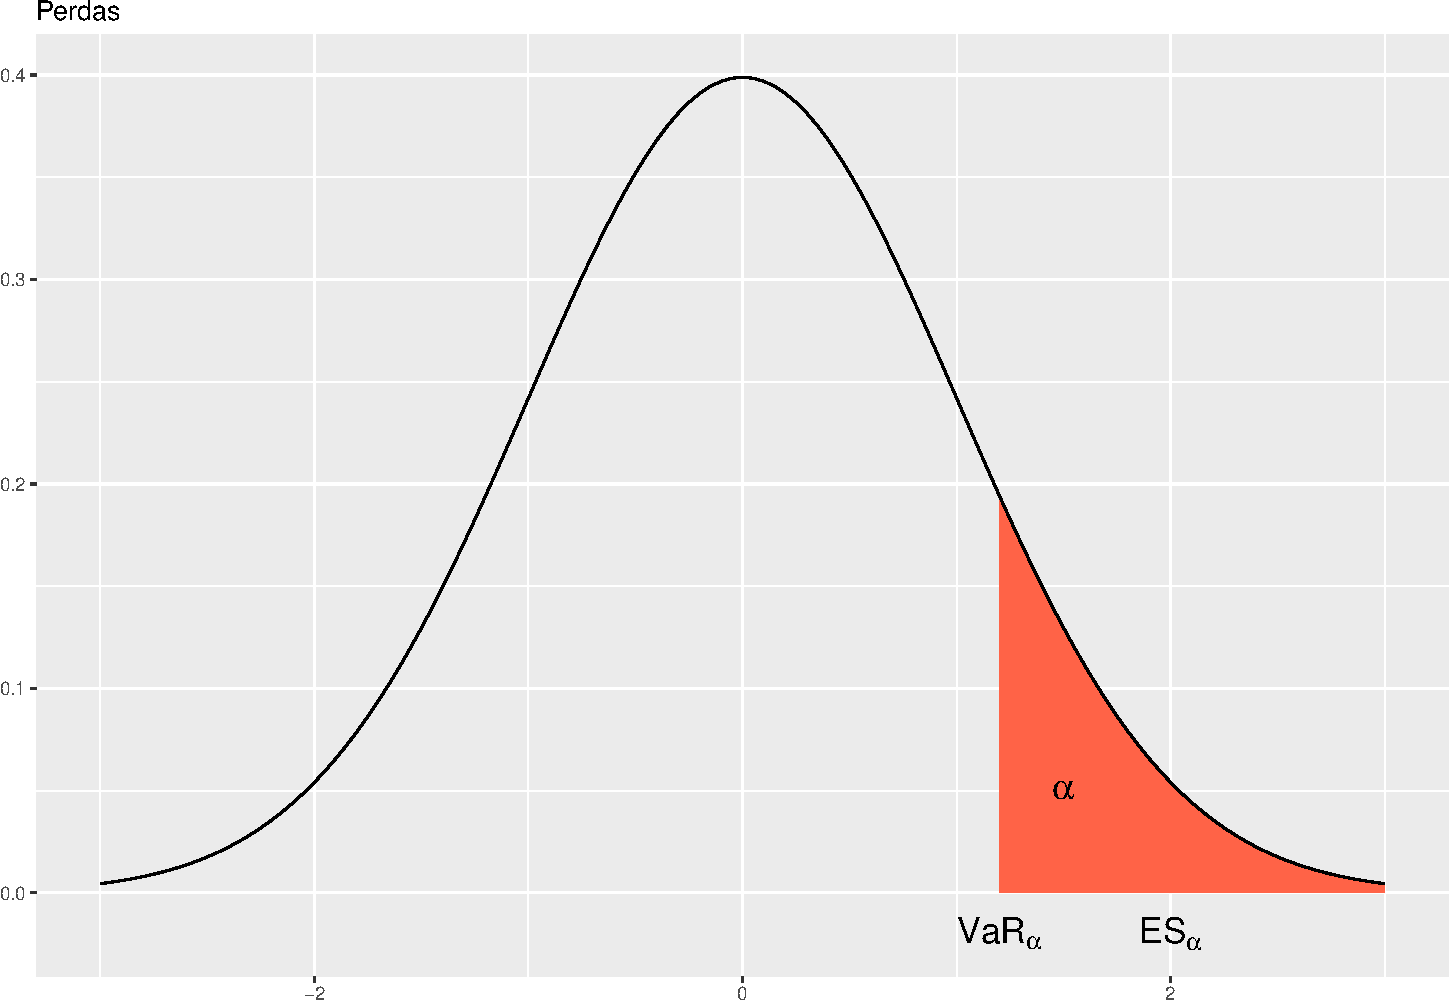
\includegraphics{artigo-apresentacao_files/figure-beamer/var-1.pdf}

\end{frame}

\section{Fundamentação Teórica}\label{fundamentacao-teorica}

\begin{frame}{Fatos estilizados}

Séries temporais de retornos possuem as seguintes características:

\begin{itemize}
\item
  Ausência de autocorrelação. Componente AR é fraco.
\item
  Grande autocorrelação nos retornos absolutos ou retornos ao quadrado.
\item
  Agrupamento (\emph{Clusters}) de volatilidade.
\item
  Persistência nas autocorrelações dos retornos ao quadrado.
\item
  Distribuição incondicional com caudas longas (leptocúrticas).
\item
  Distribuição condicional com algum grau de leptocurtose.
\item
  Assimetria entre ganhos e perdas.
\end{itemize}

\end{frame}

\begin{frame}{Fatos estilizados}

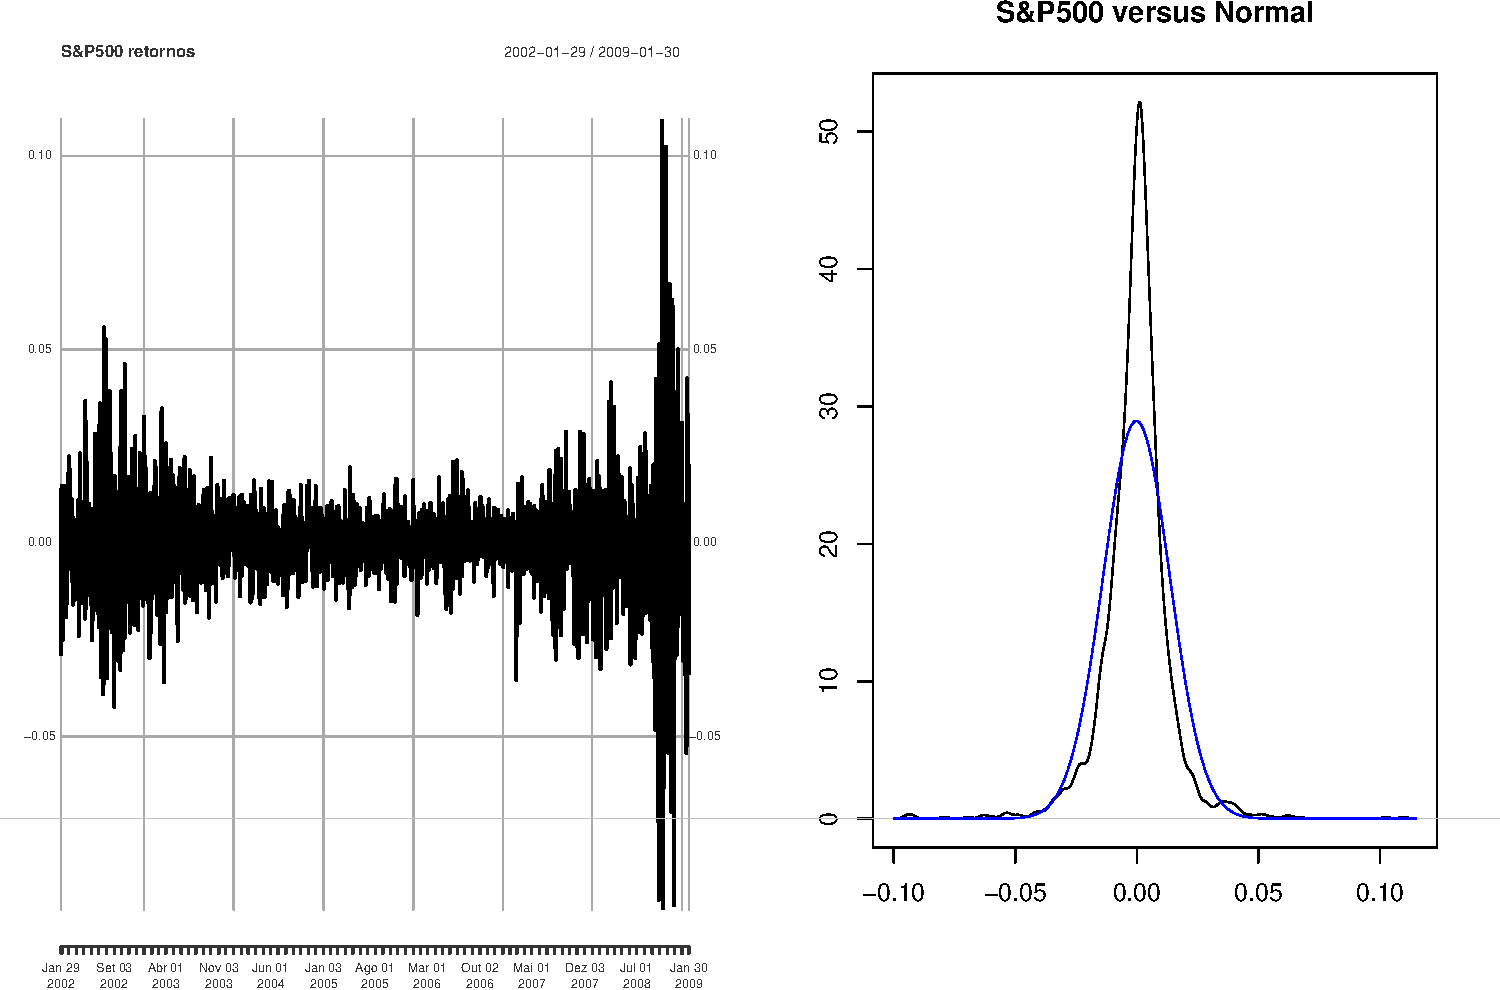
\includegraphics{artigo-apresentacao_files/figure-beamer/sp500ret-1.pdf}

\end{frame}

\begin{frame}{Modelos GARCH}

\begin{itemize}
\item
  Modelos GARCH, Bollerslev (1986) lidam com a heteroscedasticidade
  condicional encontrada nas séries financeiras.
\item
  Propriedades desejáveis: leptocurtose e autocorrelação na variância
\item
  O modelo GARCH exponencial ou eGARCH de Nelson (1991) lida também com
  o efeito alavancagem.
\end{itemize}

\begin{align*}
    L_t=&\mu+ \sum_{i=1}^r\phi_i L_{t-i}+ \sum\limits_{j=1}^{s}\theta_j\epsilon_{t-j} +\epsilon_t \\
    \ln(\sigma_t^2)=&\omega+ \sum\limits_{i=1}^{p}(\alpha_i Z_{t-i}+ \gamma_i(|Z_{t-i}|-E|Z_{t-i}|))+ \sum\limits_{j=1}^{q}\beta_j \ln(\sigma_{t-j}^2) \\
    \epsilon_t=&\sigma_t Z_t
\end{align*}

\end{frame}

\begin{frame}{Teoria do valor extremo}

\begin{itemize}
\tightlist
\item
  O método peaks-over-treshold modela a distribuição dos excessos acima
  de um determinado limiar.
\end{itemize}

\textbf{Definição} {[}Distribuição dos excessos{]}: Seja \emph{X} uma
variável aleatória com função de distribuição \(F \in MDA(H_\xi)\). A
distribuição dos excessos sobre um limiar \emph{u} tem a função de
Distribuição Generalizada de Pareto - GPD:

\begin{equation*}
  G_{\xi,\beta(u)}(X) = 
  \begin{cases}
    1- \left(1+ \frac{\xi x}{\beta(u)} \right)^{-\frac{1}{\xi}}, & \xi \neq 0,\\
    1-exp\left(-\frac{x}{\beta(u)}\right), & \xi = 0,\\
  \end{cases}
\end{equation*}

Os parâmetros \(\xi\) e \(\beta\) são conhecidos respectivamente como
parâmetros de forma e escala da distribuição.

\end{frame}

\begin{frame}{Teoria do valor extremo}

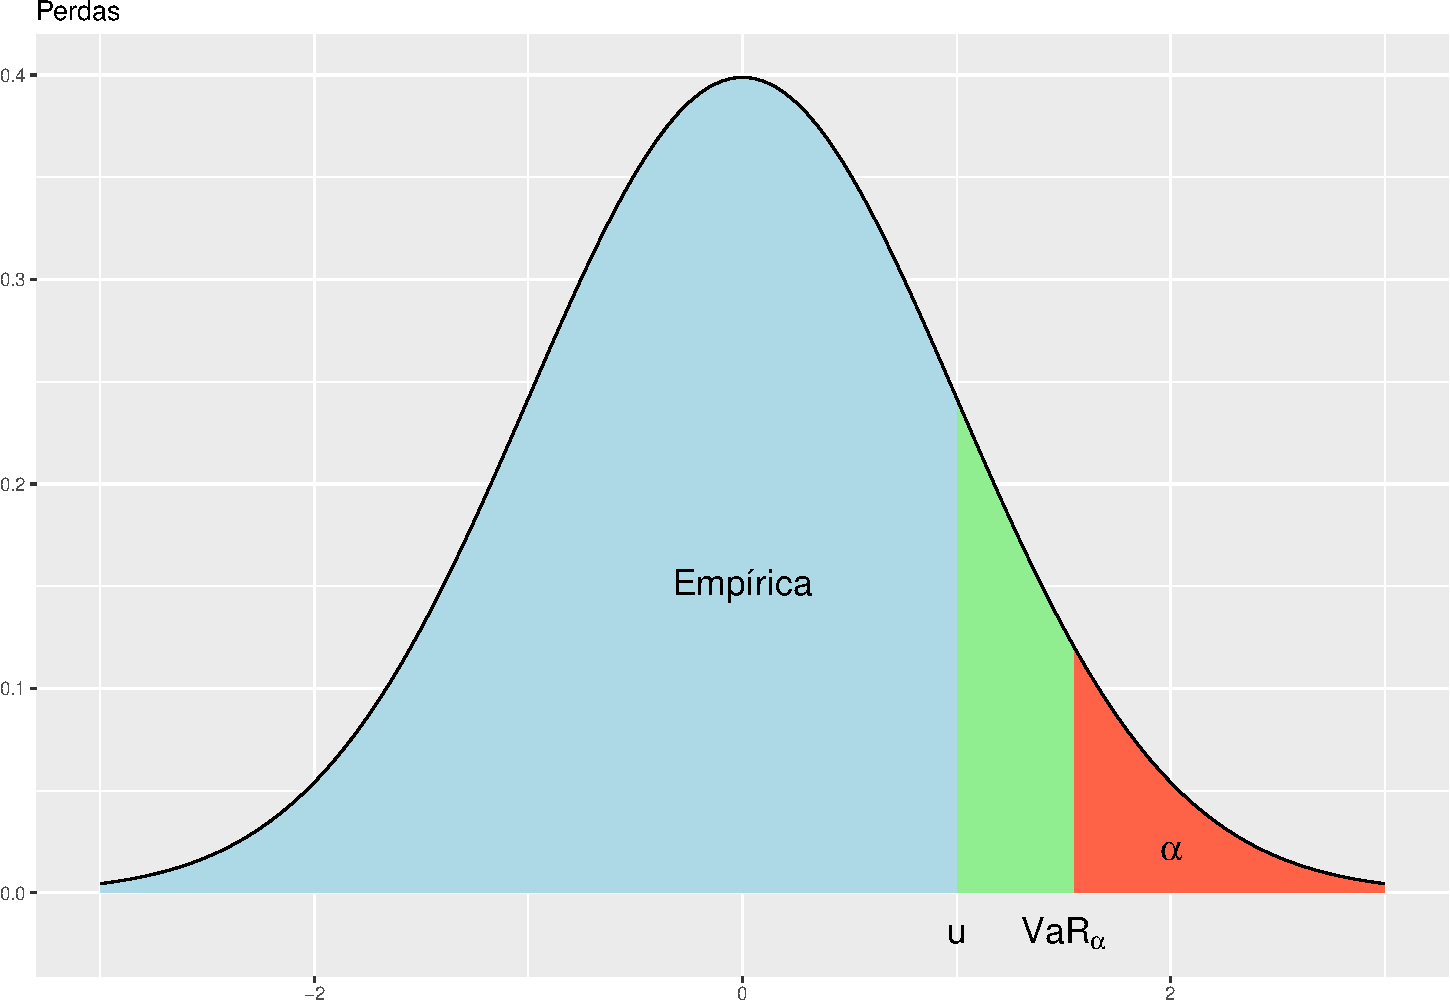
\includegraphics{artigo-apresentacao_files/figure-beamer/pot-1.pdf}

\end{frame}

\section{Modelo}\label{modelo}

\begin{frame}{Modelo eGARCH-EVT}

\begin{itemize}
\tightlist
\item
  Seguiremos os passos propostos por McNeil and Frey (2000).
\item
  Nosso modelo completo para as medidas de risco \(VaR_\alpha\) e
  \(ES_\alpha\) condicionais dada a distribuição de perdas \(L_t\) de um
  ativo será, portanto:
\end{itemize}

\begin{align*}
L_t=&\mu+ \phi_1 L_{t-1}+ \epsilon_t \\
\epsilon_t=&\sigma_t Z_t\\
\ln(\sigma_t^2)=&\omega+ \sum_{i=1}^{2}(\alpha_i Z_{t-i}+ \gamma_i(|Z_{t-i}|-E|Z_{t-i}|))+ \beta_1 \ln(\sigma_{t-1}^2) \\
Z_t\sim &\mathcal{D}(0,1) \text{ e } \mathcal{D} \in MDA(H_\xi)
\end{align*}

\end{frame}

\begin{frame}{VaR e ES parametrizados}

\begin{itemize}
\tightlist
\item
  Nossas medidas de risco neste modelo condicional serão:
\end{itemize}

\begin{align*}
VaR_\alpha^t=&\mu_{t+1}+\sigma_{t+1}z_\alpha, \\
ES_\alpha^t=&\mu_{t+1}+\sigma_{t+1}E[Z | Z>z_\alpha]
\end{align*}

onde \(z_\alpha\) é o quantil \(\alpha\) das inovações \emph{Z}.

\end{frame}

\section{Resultados}\label{resultados}

\begin{frame}{VaR condicional estimado}

\begincols

\begincol{.65\textwidth}

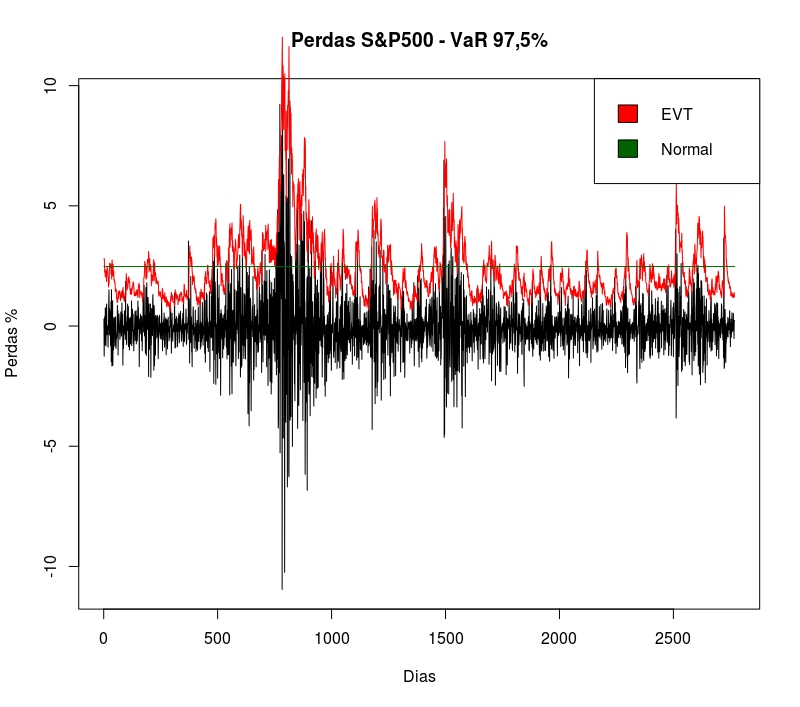
\includegraphics{artigo-apresentacao-var.jpeg}

\endcol

\begincol{.31\textwidth}


% Table created by stargazer v.5.2 by Marek Hlavac, Harvard University. E-mail: hlavac at fas.harvard.edu
% Date and time: Qua, Nov 15, 2017 - 09:17:48
\begin{table}[!htbp] \centering 
%  \caption{} 
  \label{} 
\tiny 
\begin{tabular}{@{\extracolsep{5pt}} ccc} 
\\[-1.8ex]\hline 
\hline \\[-1.8ex] 
Modelo & Violações & Proporção \\ 
\hline \\[-1.8ex] 
EVT & $69$ & $2.493$ \\ 
Normal & $84$ & $3.035$ \\ 
\hline \\[-1.8ex] 
\end{tabular} 
\end{table} 


\endcol

\endcols

\end{frame}

\begin{frame}{Referências}

\hypertarget{refs}{}
\hypertarget{ref-Acerbi2001}{}
Acerbi, Carlo, and Dirk Tasche. 2001. ``Expected Shortfall: A Natural
Coherent Alternative to Value at Risk.'' \emph{Economic Notes} 31 (2):
379--88.
doi:\href{https://doi.org/10.1111/1468-0300.00091}{10.1111/1468-0300.00091}.

\hypertarget{ref-Bollerslev1986}{}
Bollerslev, Tim. 1986. ``Generalized autoregressive conditional
heteroskedasticity.'' \emph{Journal of Econometrics} 31 (3): 307--27.
doi:\href{https://doi.org/10.1016/0304-4076(86)90063-1}{10.1016/0304-4076(86)90063-1}.

\hypertarget{ref-McNeil2000}{}
McNeil, Alexander J, and Rüdiger Frey. 2000. ``Estimation of
tail-related risk measures for heteroscedastic financial time series: an
extreme value approach.'' \emph{Journal of Empirical Finance} 7 (3-4):
271--300.
doi:\href{https://doi.org/10.1016/s0927-5398(00)00012-8}{10.1016/s0927-5398(00)00012-8}.

\hypertarget{ref-Nelson1991}{}
Nelson, Daniel B. 1991. ``Conditional Heteroskedasticity in Asset
Returns: A New Approach.'' \emph{Econometrica: Journal of the
Econometric Society}. JSTOR, 347--70.

\end{frame}

\end{document}
